% =====================================================================
%  Rapport de stage — RAGLab
%  Système de question-réponse documentaire (RAG) sur documents bancaires
%
%  Compilation : pdflatex (2 passes) — aucune dépendance exotique.
%  Les termes arabes sont translittérés dans ce fichier afin qu'il compile
%  avec pdflatex sans police arabe ; la version Markdown et le PDF joint
%  conservent l'écriture arabe.
%
%  CHAMP À PERSONNALISER : \EtudiantNom (voir le bloc \newcommand ci-dessous).
% =====================================================================
\documentclass[a4paper,12pt]{report}
\usepackage[utf8]{inputenc}
\usepackage[T1]{fontenc}
\usepackage[french]{babel}
\usepackage{graphicx}
\usepackage{geometry}
\usepackage{setspace}
\usepackage{hyperref}
\usepackage{float}
\usepackage{array}
\usepackage{booktabs}
\usepackage{xcolor}
\usepackage{titlesec}
\usepackage{fancyhdr}

\geometry{margin=2.4cm}
\setstretch{1.35}
\graphicspath{{./}}

% ============================================================
%  INFORMATIONS PERSONNELLES
% ============================================================
\newcommand{\EtudiantNom}{[[INTERN_NAME]]}
\newcommand{\EcoleNom}{École supérieure privée d'ingénierie et de technologie}
\newcommand{\EntrepriseNom}{Al Baraka Bank}
\newcommand{\EncadrantNom}{Ahlem BENHADDOUD}
\newcommand{\StagePeriode}{Du 1\textsuperscript{er} août au 1\textsuperscript{er} octobre 2026}
\newcommand{\AnneeUniv}{2025 -- 2026}
\newcommand{\SujetStage}{Conception et évaluation d'un système de question-réponse
documentaire (RAG) appliqué à des documents bancaires arabes}

\definecolor{genone}{HTML}{2F6FD0}
\definecolor{genpivot}{HTML}{B57A14}
\definecolor{gentwo}{HTML}{1F7A5C}
\definecolor{genlast}{HTML}{B3205A}

\titleformat{\chapter}[display]{\bfseries\Large}{}{0pt}{\Large}
\titlespacing{\chapter}{0pt}{-10pt}{14pt}
\titleformat{\section}{\bfseries\large}{\thesection}{0.6em}{}
\titleformat{\subsection}{\bfseries\normalsize}{\thesubsection}{0.6em}{}

\pagestyle{fancy}
\fancyhf{}
\fancyhead[L]{\small Rapport de stage — RAGLab}
\fancyhead[R]{\small \thepage}
\renewcommand{\headrulewidth}{0.3pt}

\begin{document}

% ====================== PAGE DE GARDE ======================
\begin{titlepage}
\centering
\vspace*{0.6cm}
{\large \textbf{République Tunisienne}}\\[0.2cm]
{\normalsize \EcoleNom}\\[0.9cm]
{\large \textbf{\SujetStage}}\\[1.1cm]

\begin{tabular}{rl}
\textbf{Réalisé par :} & \EtudiantNom \\[0.15cm]
\textbf{Entreprise d'accueil :} & \EntrepriseNom \\[0.15cm]
\textbf{Période :} & \StagePeriode \\[0.15cm]
\textbf{Encadrante :} & \EncadrantNom \\[0.15cm]
\textbf{Année universitaire :} & \AnneeUniv \\
\end{tabular}

\vfill
{\small \textit{Rapport d'immersion en entreprise — version du 5 octobre 2026}}
\end{titlepage}

% ====================== DÉDICACES / REMERCIEMENTS ======================
\chapter*{Dédicaces}
\addcontentsline{toc}{chapter}{Dédicaces}
Je dédie ce travail à ma famille, pour son soutien constant tout au long de ce parcours,
et à toutes les personnes qui m'ont encouragé à transformer une idée en système mesuré.

\chapter*{Remerciements}
\addcontentsline{toc}{chapter}{Remerciements}
Mes remerciements vont d'abord à \EncadrantNom, pour l'encadrement rigoureux, la disponibilité
et les décisions de cadrage qui ont structuré ce travail. Je remercie également l'équipe de
\EntrepriseNom pour l'accueil, les documents mis à disposition et les retours d'exploitation
qui ont permis de détecter des défauts invisibles en test. Je remercie enfin les enseignants de
\EcoleNom pour la formation qui a rendu ce projet possible.

\chapter*{Résumé}
\addcontentsline{toc}{chapter}{Résumé}
Ce rapport rend compte d'un stage de fin d'études consacré à la conception, à la construction et
à l'évaluation de \textbf{RAGLab}, un système de question-réponse documentaire (RAG) appliqué à
des documents bancaires arabes. Le système répond uniquement à partir d'un corpus de quatre
documents réels, exige que chaque affirmation soit adossée à une citation \emph{littérale} dont
tous les nombres figurent dans la source, et refuse de répondre — en expliquant ce qui manque —
lorsque la preuve est insuffisante. L'architecture a évolué en cours de projet : une première
génération de type laboratoire de recherche d'information a été remplacée, après un pivot
méthodologique, par une architecture en quatre couches gouvernées — structure, connaissance,
compréhension, livraison et audit. Les résultats mesurés montrent l'apport du découpage structurel
(+20 points de hit@1 : 51 $\rightarrow$ 71), la supériorité de la recherche dense sur la fusion
BM25 sur ce corpus, un index d'unités de connaissance à 100/100/100 sur les questions de loi, et
un accord inter-modèles de 0,720 avec des citations identiques à contexte fixé.

\textbf{Mots-clés :} RAG · recherche d'information · documents bancaires arabes · ancrage des
citations · suffisance de preuve · évaluation mesurée.

\chapter*{Executive summary (English)}
\addcontentsline{toc}{chapter}{Executive summary (English)}
\textbf{Context and objective.} This report documents the design, implementation and measurement
of \textbf{RAGLab}, a document-grounded question-answering system (Retrieval-Augmented Generation)
built for Arabic-language banking documents. An assistant that answers questions about regulatory
and internal documents must never invent figures or rules, and must be able to show the exact
passage it relied on. The project therefore optimised for traceability and honest refusal rather
than fluent prose.

\textbf{What was built.} The work went through two architectures. \emph{Generation 1} was a flat
retrieval laboratory: several embedding providers, machine-translated query variants, three
retrieval modes (dense, BM25 fusion, score blending) and a citation gate, compared by measured
A/B runs. \emph{The pivot} (24--28 September 2026) followed an external target-state report: the
corpus was reduced to four real documents, every step became an owner-gated plan, and
\emph{Generation 2} added four explicit layers — corpus/structure, knowledge (198 law units,
77 cross-references, 53 structured number records, governance axes), understanding (intent,
evidence plan, sufficiency, decomposition, bounded interrogation) and delivery (citation gate,
PII scrubbing, audit trail).

\textbf{Key results.} Structural chunking beats token-window chunking on the live arm
(hit@1/3/5: 51/64/71 $\rightarrow$ \textbf{71/80/87}); dense retrieval beats BM25 fusion and
blending (71/80/87 vs 71/80/82 vs 62/80/84), so the vector arm stayed the default. The unit index
answers the law questions perfectly (100/100/100 vs 67/92/92). With retrieval fixed, 72\,\% of
outcomes agree between two answer models and cited sources are identical whenever both answer.
The final iteration rebuilt the question-to-corpus topic link, fixed a live defect that kept the
guided retrieval round from running in the deployed service, fixed a French intent-classification
root cause, blocked duplicate document pushes by content hash, and disclosed re-aimed answers.

\textbf{Limits.} The pipeline validates that quotes and numbers exist in the cited sources; it
does not prove that a claim is \emph{entailed} by them. There is no similarity threshold, the
service is a single stateful worker, updates require re-ingestion, and the evaluation sets are
small and correlated. The system is \textbf{not production-ready for a banking service}.

\tableofcontents

% ====================== INTRODUCTION ======================
\chapter{Introduction générale}

Les établissements bancaires produisent et consomment une masse de textes réglementaires et
procéduraux : lois, circulaires de la banque centrale, guides internes, supports de formation.
Retrouver une information fiable dans ces documents est un exercice coûteux, et le confier à un
modèle de langage « brut » est dangereux : un modèle génératif répond toujours, même lorsqu'il ne
sait pas, et rien ne distingue une phrase recopiée d'une phrase inventée.

Le stage dont ce rapport rend compte a porté sur la conception, la construction et l'évaluation
d'un système de \textbf{question-réponse documentaire} (RAG, \emph{Retrieval-Augmented
Generation}) sur un corpus bancaire réel en langue arabe. Le projet, baptisé \textbf{RAGLab},
poursuit trois objectifs :

\begin{enumerate}
  \item \textbf{Traçabilité.} Chaque affirmation de la réponse doit être adossée à un extrait
        littéral du document cité, et chaque nombre avancé doit figurer dans cet extrait.
  \item \textbf{Refus honnête.} Quand la preuve manque, le système doit refuser de répondre — en
        expliquant ce qui manque — plutôt que de produire une réponse plausible.
  \item \textbf{Mesure.} Aucun choix d'architecture n'est retenu sans une comparaison mesurée,
        reproductible, et un critère de décision explicite.
\end{enumerate}

Le rapport suit le déroulement réel du travail. Le chapitre 1 présente le contexte, le problème
métier et la méthode. Le chapitre 2 situe les choix techniques par rapport à l'état de l'art du
RAG. Le chapitre 3 décrit l'architecture — en montrant qu'elle a \textbf{changé en cours de
route} : une première génération de type laboratoire, puis un pivot méthodologique, puis une
seconde génération organisée en couches, dont la dernière évolution est mise en évidence. Le
chapitre 4 présente les mesures, les résultats et les limites.

Une remarque de méthode : le projet a été développé sur un dépôt versionné, avec une discipline de
mesure et de revue constante. Les chiffres cités sont reproductibles à partir du dépôt et leur
provenance est indiquée en annexe B.

% ====================== CHAPITRE 1 ======================
\chapter{Contexte et cadrage du projet}

\section{L'entreprise d'accueil}
Le stage s'est déroulé au sein d'\textbf{Al Baraka Bank}, banque islamique de la place tunisienne.
Ses activités et ses produits s'inscrivent dans le cadre de la \textbf{loi n\textsuperscript{o}
2016-48 du 11 juillet 2016 relative aux banques et aux établissements financiers}, l'un des
documents du corpus de ce projet.

\emph{TODO-ENTREPRISE} — compléter si nécessaire les éléments factuels d'entreprise (date de
création, effectif, réseau, périmètre d'activité) à partir des sources officielles de la banque.

\paragraph{Environnement de travail.} Le projet a été mené dans un environnement de développement
individuel : Python 3.11, un dépôt Git, un service local conteneurisé, et une intégration continue
utilisée à la fois comme porte de qualité et comme banc de mesure des modèles réels. Deux
contraintes matérielles ont structuré la méthode : l'absence d'accès réseau vers les fournisseurs
de modèles depuis le poste de développement (les mesures « live » sont donc exécutées dans
l'intégration continue) et l'absence de GPU (d'où le recours à des modèles servis par API).

\section{Problématique métier}
Le corpus réuni pour l'évaluation est composé de quatre documents réels, tous en arabe :

\begin{table}[H]
\centering
\small
\begin{tabular}{p{4.6cm}p{2.9cm}p{6.4cm}}
\toprule
\textbf{Document} & \textbf{Nature} & \textbf{Rôle dans le corpus} \\
\midrule
Loi n\textsuperscript{o} 2016-48 (11 juillet 2016) & Loi & Référence juridique supérieure
(198 articles, 11 titres) \\
Circulaire BCT n\textsuperscript{o} 2019-08 & Circulaire & Cadrage opérationnel des opérations
(20 chapitres) \\
Guide interne d'opérations bancaires islamiques & Guide interne & Politique et procédures
internes de conformité \\
Introduction à la finance islamique (\emph{Madkhal}) & Support de formation & Historique,
définitions, ordres de grandeur \\
\bottomrule
\end{tabular}
\end{table}

Trois questions concrètes ont motivé le projet.

\begin{itemize}
  \item \textbf{La question de l'utilisateur est rarement la question du document.} Un client ou
        un agent formule une demande en langage courant (« puis-je ouvrir un commerce ? ») là où
        le corpus contient des formulations techniques (\emph{al-sigha}, \emph{mahall al-aqd},
        \emph{tamwil}). La réponse doit être retrouvée malgré cet écart lexical et syntaxique.
  \item \textbf{Le multilinguisme est asymétrique.} Le corpus est arabe, mais les questions
        arrivent aussi en français et en anglais ; une question française doit pouvoir s'appuyer
        sur un passage arabe sans jamais traduire l'utilisateur ni le document.
  \item \textbf{L'erreur est coûteuse.} Dans un contexte bancaire, une réponse fausse sur un taux,
        un délai ou une sanction n'est pas une simple imprécision : c'est un risque juridique.
\end{itemize}

\section{Objectifs du stage}
\begin{enumerate}
  \item Construire une chaîne complète \emph{chargement $\rightarrow$ découpage $\rightarrow$
        vectorisation $\rightarrow$ indexation $\rightarrow$ recherche $\rightarrow$ génération
        ancrée $\rightarrow$ vérification} sur les documents réels.
  \item Ne retenir que des modèles \textbf{libres d'accès} et reproductibles, en documentant les
        mesures comparatives plutôt que les impressions.
  \item Faire du \textbf{refus explicite} un comportement de premier rang, avec une taxonomie de
        raisons.
  \item Livrer le système sous forme de \textbf{service} intégré à l'application de la banque,
        avec un contrat HTTP stable, versionné et testé.
  \item Instrumenter la qualité : tests hors ligne, intégration continue, jeux de questions gelés,
        journal d'audit.
\end{enumerate}

\section{Contraintes du projet}
\begin{table}[H]
\centering
\small
\begin{tabular}{p{6.0cm}p{8.2cm}}
\toprule
\textbf{Contrainte} & \textbf{Conséquence sur la méthode} \\
\midrule
Aucun accès réseau aux API de modèles depuis le poste & Les mesures sur modèles réels s'exécutent
en intégration continue, sur déclenchement explicite (coût maîtrisé) \\
Pas de GPU & Modèles servis par API, épinglés et versionnés \\
Corpus réel uniquement & Aucun corpus fictif dans le dépôt ; jeux de tests gelés et versionnés \\
Service en cours d'intégration & \textbf{Gel des points d'entrée HTTP} : évolution additive
seulement, avec incrément de version \\
Exigence de traçabilité & Chaque chiffre publié est rattaché à un commit, un journal ou un
identifiant d'exécution \\
\bottomrule
\end{tabular}
\end{table}

\section{Méthode de travail}
Le projet a suivi un protocole dit « \textbf{étape et plan} », adopté après le pivot du
chapitre 3. Chaque étape publie son propre plan, en huit points, avant d'écrire la moindre ligne
de code : objectif et périmètre ; entrées ; actions numérotées ; sorties ; vérification
automatique ; façon dont le donneur d'ordre teste lui-même le résultat ; critère de passage ;
point de retour.

Deux règles complètent ce protocole : la porte locale (compilation, contrôles hors ligne, tests
unitaires, inspection) doit être verte \textbf{avant} toute publication, et l'intégration continue
surveillée jusqu'au vert \textbf{après}. Les jeux de questions sont gelés : une campagne qui les
modifierait serait invalidée.

L'implémentation a été menée avec l'assistance d'un agent de codage, sous la forme d'un
\textbf{contrat de travail écrit} qui consigne les contraintes, les faits vérifiés et les pièges
déjà rencontrés. Chaque étape reste soumise à une validation humaine : l'agent propose, mesure et
documente ; les décisions d'activation appartiennent au donneur d'ordre. Cette organisation s'est
révélée décisive pour la reproductibilité : elle a permis de reprendre le projet après plusieurs
interruptions sans repartir de zéro, et d'éviter qu'un même défaut soit diagnostiqué deux fois.

% ====================== CHAPITRE 2 ======================
\chapter{État de l'art et choix techniques}

\section{Le principe du RAG et ses points de rupture}
Un système RAG combine un \textbf{système de recherche d'information} qui sélectionne des extraits
pertinents dans une base documentaire, et un \textbf{modèle de langage} qui rédige une réponse à
partir de ces extraits. Cette architecture déplace le problème plus qu'elle ne le résout : les
points de rupture sont connus et ont structuré tout le projet.

\begin{table}[H]
\centering
\small
\begin{tabular}{p{3.5cm}p{5.0cm}p{5.7cm}}
\toprule
\textbf{Point de rupture} & \textbf{Symptôme observé} & \textbf{Réponse apportée} \\
\midrule
Découpage arbitraire & Une définition coupée en deux devient inutilisable & Découpage structurel
(§3.4.1) \\
Écart lexical & La question dit « murabaha », le document dit « al-murabaha » & Normalisation arabe
partagée, ponts entre systèmes d'écriture, interrogation bornée \\
Faux positifs de similarité & Les extraits remontés sont hors sujet sans que rien ne le signale &
État de suffisance déterministe, refus explicite \\
Hallucination & Une phrase correcte énonce un chiffre inventé & Contrôle des citations \emph{et}
des nombres (§3.4.4) \\
Perte de traçabilité & Impossible de vérifier ce que le modèle a lu & Citations littérales,
identifiants de fragments, journal d'audit \\
Régressions silencieuses & Une amélioration locale dégrade un autre cas & Jeux gelés, mesures
appariées \\
\bottomrule
\end{tabular}
\end{table}

\section{Le découpage : de la fenêtre fixe au découpage structurel}
Le \textbf{découpage à fenêtre fixe} coupe le texte tous les $N$ tokens avec un recouvrement ; il
est simple, uniforme, et aveugle à la structure. Le \textbf{découpage structurel} respecte les
frontières du document (titres, articles, paragraphes, tableaux) ; il produit des unités de sens,
au prix d'une analyse préalable.

Le projet a implémenté les deux, puis les a mesurés. Le mode historique \texttt{size}
(220 tokens, 40 de recouvrement) reste disponible ; le mode \texttt{restructure}, devenu la
valeur par défaut, met en œuvre un enchaînement en trois étapes :

\begin{enumerate}
  \item \textbf{Normalisation sémantique} — nettoyage des en-têtes de gazette, suppression des
        en-têtes répétés, extraction des marqueurs de section (\emph{al-fasl}, \emph{al-unwan},
        \emph{al-bab}), reconstruction de l'ordre visuel des lignes arabes issues des PDF.
  \item \textbf{Enrichissement par fil d'Ariane} — injection, au-dessus de chaque sous-titre et de
        chaque tableau, d'une ligne de contexte \texttt{h1 > h2 > h3}.
  \item \textbf{Découpage structurel récursif} — séparation selon une hiérarchie de séparateurs
        (\texttt{\textbackslash n\# }, \texttt{\textbackslash n\#\# },
        \texttt{\textbackslash n\#\#\# }, ligne vide, saut de ligne, espace) au budget habituel
        de 220/40 tokens.
\end{enumerate}

Une étape de \textbf{réparation linguistique} des textes extraits s'y ajoute : les PDF de textes
juridiques arabes ressortent en ordre visuel avec des chiffres corrompus, ce qui rend le corpus
inutilisable en l'état.

\section{Les représentations vectorielles}
Les modèles d'\emph{embeddings} multilingues projettent un texte dans un espace où la proximité
traduit la proximité de sens. Pour l'arabe, deux difficultés dominent : la morphologie riche
(préfixes, suffixes, formes définies) et la coexistence de plusieurs systèmes d'écriture dans les
mêmes questions (les termes techniques sont souvent écrits en caractères latins).

Plusieurs fournisseurs ont été comparés — Google, Jina, HuggingFace, NVIDIA — avant de
\textbf{fixer} le couple retenu : \texttt{nvidia/nemotron-3-embed-1b}, en dimension native 2048.
Ce choix fige l'espace vectoriel, ce qui autorise une vérification forte : chaque index stocke une
\textbf{empreinte} du modèle et du découpage qui l'a produit, et une recherche incohérente avec
cette empreinte est refusée avant tout appel de modèle.

\section{La recherche : dense, lexicale, hybride}
Trois stratégies ont été implémentées et mesurées :
\begin{itemize}
  \item \textbf{vectorielle (dense)} — similarité cosinus sur les vecteurs ;
  \item \textbf{RRF} — fusion par rang réciproque (constante 60) entre la recherche dense et un
        index lexical BM25 ($k_1 = 1{,}5$ ; $b = 0{,}75$) ;
  \item \textbf{blend} — fusion par score, $\lambda \cdot \text{cosinus} + (1-\lambda) \cdot
        \text{BM25 normalisé}$, $\lambda = 0{,}7$.
\end{itemize}
La mesure a tranché (§4.4) : la fusion lexicale n'apporte pas de gain net et dégrade le français.
Le mode dense reste la valeur par défaut, les deux autres restant des options explicites.

\section{L'ancrage : contrôle des citations et suffisance}
La contribution la plus significative du projet n'est pas la recherche mais la
\textbf{vérification}. Le modèle ne renvoie pas du texte libre : il doit produire un objet JSON de
type \texttt{grounded-v1}, où chaque affirmation porte une ou plusieurs preuves, chacune étant une
citation \textbf{littérale} d'un extrait fourni. Trois contrôles déterministes s'appliquent :
\begin{enumerate}
  \item \textbf{Appartenance des citations} — après normalisation (arabe, casse, espaces), chaque
        citation doit être une sous-chaîne de l'extrait cité ;
  \item \textbf{Contrôle numérique} — tout nombre en chiffres présent dans une affirmation doit
        apparaître dans ses citations, séparateurs de milliers et chiffres arabo-indiens inclus ;
  \item \textbf{Contrôle de politique} — la source citée doit avoir été réellement récupérée,
        appartenir aux documents autorisés et, lorsque l'axe de vigueur est renseigné, être en
        vigueur.
\end{enumerate}
En amont de la génération, une couche déterministe de \textbf{suffisance} confronte le besoin de
preuve (dérivé de l'intention de la question) au contenu réellement récupéré et produit quatre
états : suffisant, insuffisant, contradictoire, indéterminé. C'est cet état — et non un score de
similarité — qui décide si le système répond, refuse, ou tente une seule réinterprétation bornée.

\section{L'évaluation}
Le projet mesure la \textbf{retrouvabilité} (hit@1, hit@3, hit@5 : le document et l'extrait
attendus apparaissent-ils parmi les $k$ premiers résultats) et le \textbf{comportement final}
(réponse ancrée, refus motivé). Deux jeux gelés servent de référence : 50 cas (10 verbatim,
20 paraphrases, 15 transfrontaliers, 5 hors périmètre) et 10 cas arabes couvrant cinq catégories
cibles (langage familier, synonymes, demande implicite, demande composée, ambiguïté).

Trois règles rendent les comparaisons défendables : les chiffres comparés sont mesurés dans la
\textbf{même exécution} ; les comparaisons inter-exécutions portent une tolérance de $\pm 2$ points
(les modèles servis ne sont pas bit-reproductibles) ; un jeu gelé n'est jamais modifié pour
améliorer un résultat.

\section{Les modèles retenus}
Une comparaison mesurée de modèles gratuits (13 vérifications de développement, 18 vérifications
en aveugle, 3 scénarios d'injection) a conduit à figer un couple unique :

\begin{table}[H]
\centering
\small
\begin{tabular}{p{2.6cm}p{5.3cm}p{6.3cm}}
\toprule
\textbf{Rôle} & \textbf{Fournisseur / modèle} & \textbf{Justification} \\
\midrule
Vectorisation & NVIDIA \texttt{nemotron-3-embed-1b} (2048 dimensions) & Qualité mesurée sur le
corpus arabe, dimension native élevée, mise en cache possible \\
Réponse & xKiro \texttt{qwen/qwen3.8-max:free} & Meilleur taux de citations conformes au contrat
\texttt{grounded-v1}, contrôle de prix en direct \\
\bottomrule
\end{tabular}
\end{table}

Deux décisions renforcent la reproductibilité : \textbf{aucun repli} n'est autorisé (un modèle
différent provoque une erreur explicite, pas une dégradation silencieuse) et la traduction
automatique des requêtes est \textbf{retirée} (mesurée et documentée comme historique).

\section{L'écosystème technique}
\begin{table}[H]
\centering
\small
\begin{tabular}{p{3.2cm}p{5.6cm}p{5.4cm}}
\toprule
\textbf{Brique} & \textbf{Choix} & \textbf{Alternative écartée} \\
\midrule
Orchestration & Code Python explicite & LangChain / LlamaIndex : boîte noire, dépendances \\
Base vectorielle & ChromaDB local, persistant, cosinus & Base cloud : coût, données bancaires \\
Appels HTTP & \texttt{urllib} de la bibliothèque standard & SDK fournisseurs : dépendances \\
Service & FastAPI + uvicorn & — \\
Découpage & \texttt{tiktoken} (\texttt{cl100k\_base}) + estimation de repli & — \\
PDF / DOCX & \texttt{pypdf} ; lecture directe OOXML & SDK bureautiques \\
Tests / CI & \texttt{unittest} + GitHub Actions (7 scénarios) & — \\
\bottomrule
\end{tabular}
\end{table}

Le dépôt ne contient \textbf{ni framework d'orchestration, ni base vectorielle externe, ni SDK de
fournisseur} : cette contrainte facilite l'audit et l'exploitation chez un hébergeur interne.

% ====================== CHAPITRE 3 ======================
\chapter{Architecture et implémentation}

\section{Vue d'ensemble : deux générations et un pivot}

\begin{figure}[H]
\centering
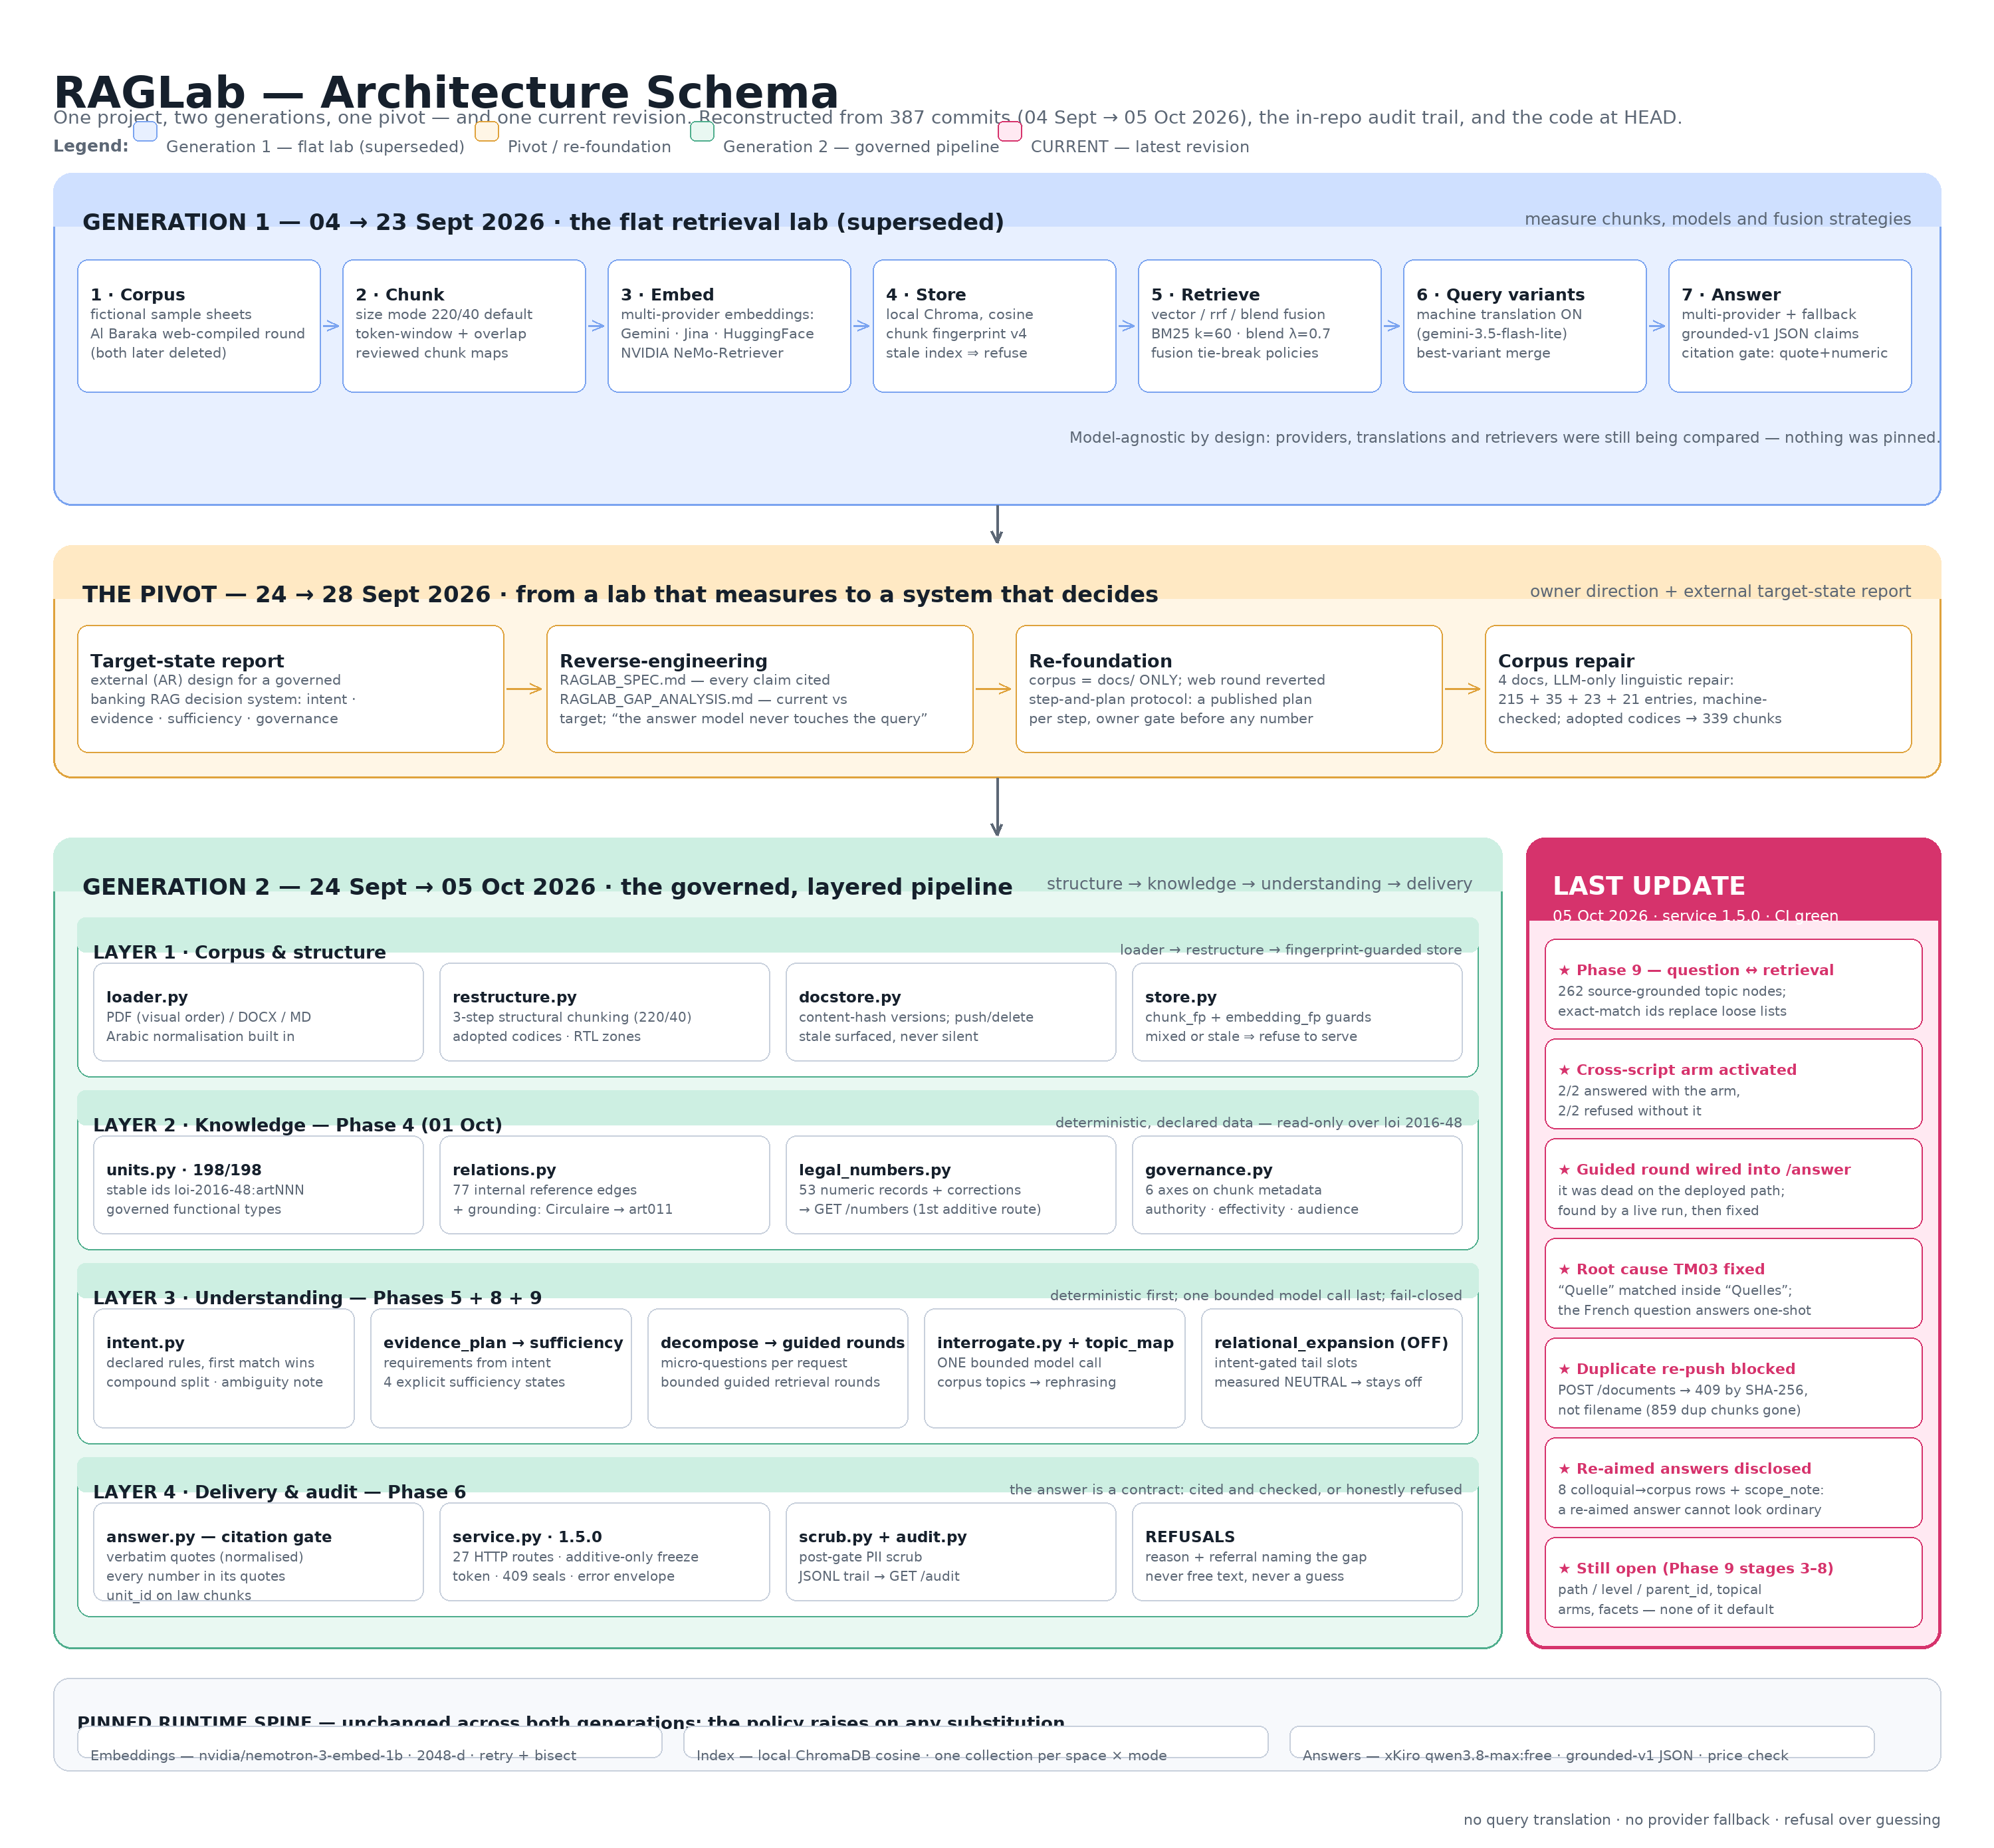
\includegraphics[width=\textwidth]{architecture_schema.png}
\caption{Schéma d'architecture — génération 1 (laboratoire plat), pivot, génération 2 en quatre
couches, et encadré \emph{LAST UPDATE} isolant la dernière évolution. Le fichier vectoriel
\texttt{architecture\_schema.svg} donne la même figure en qualité imprimable.}
\end{figure}

\begin{figure}[H]
\centering
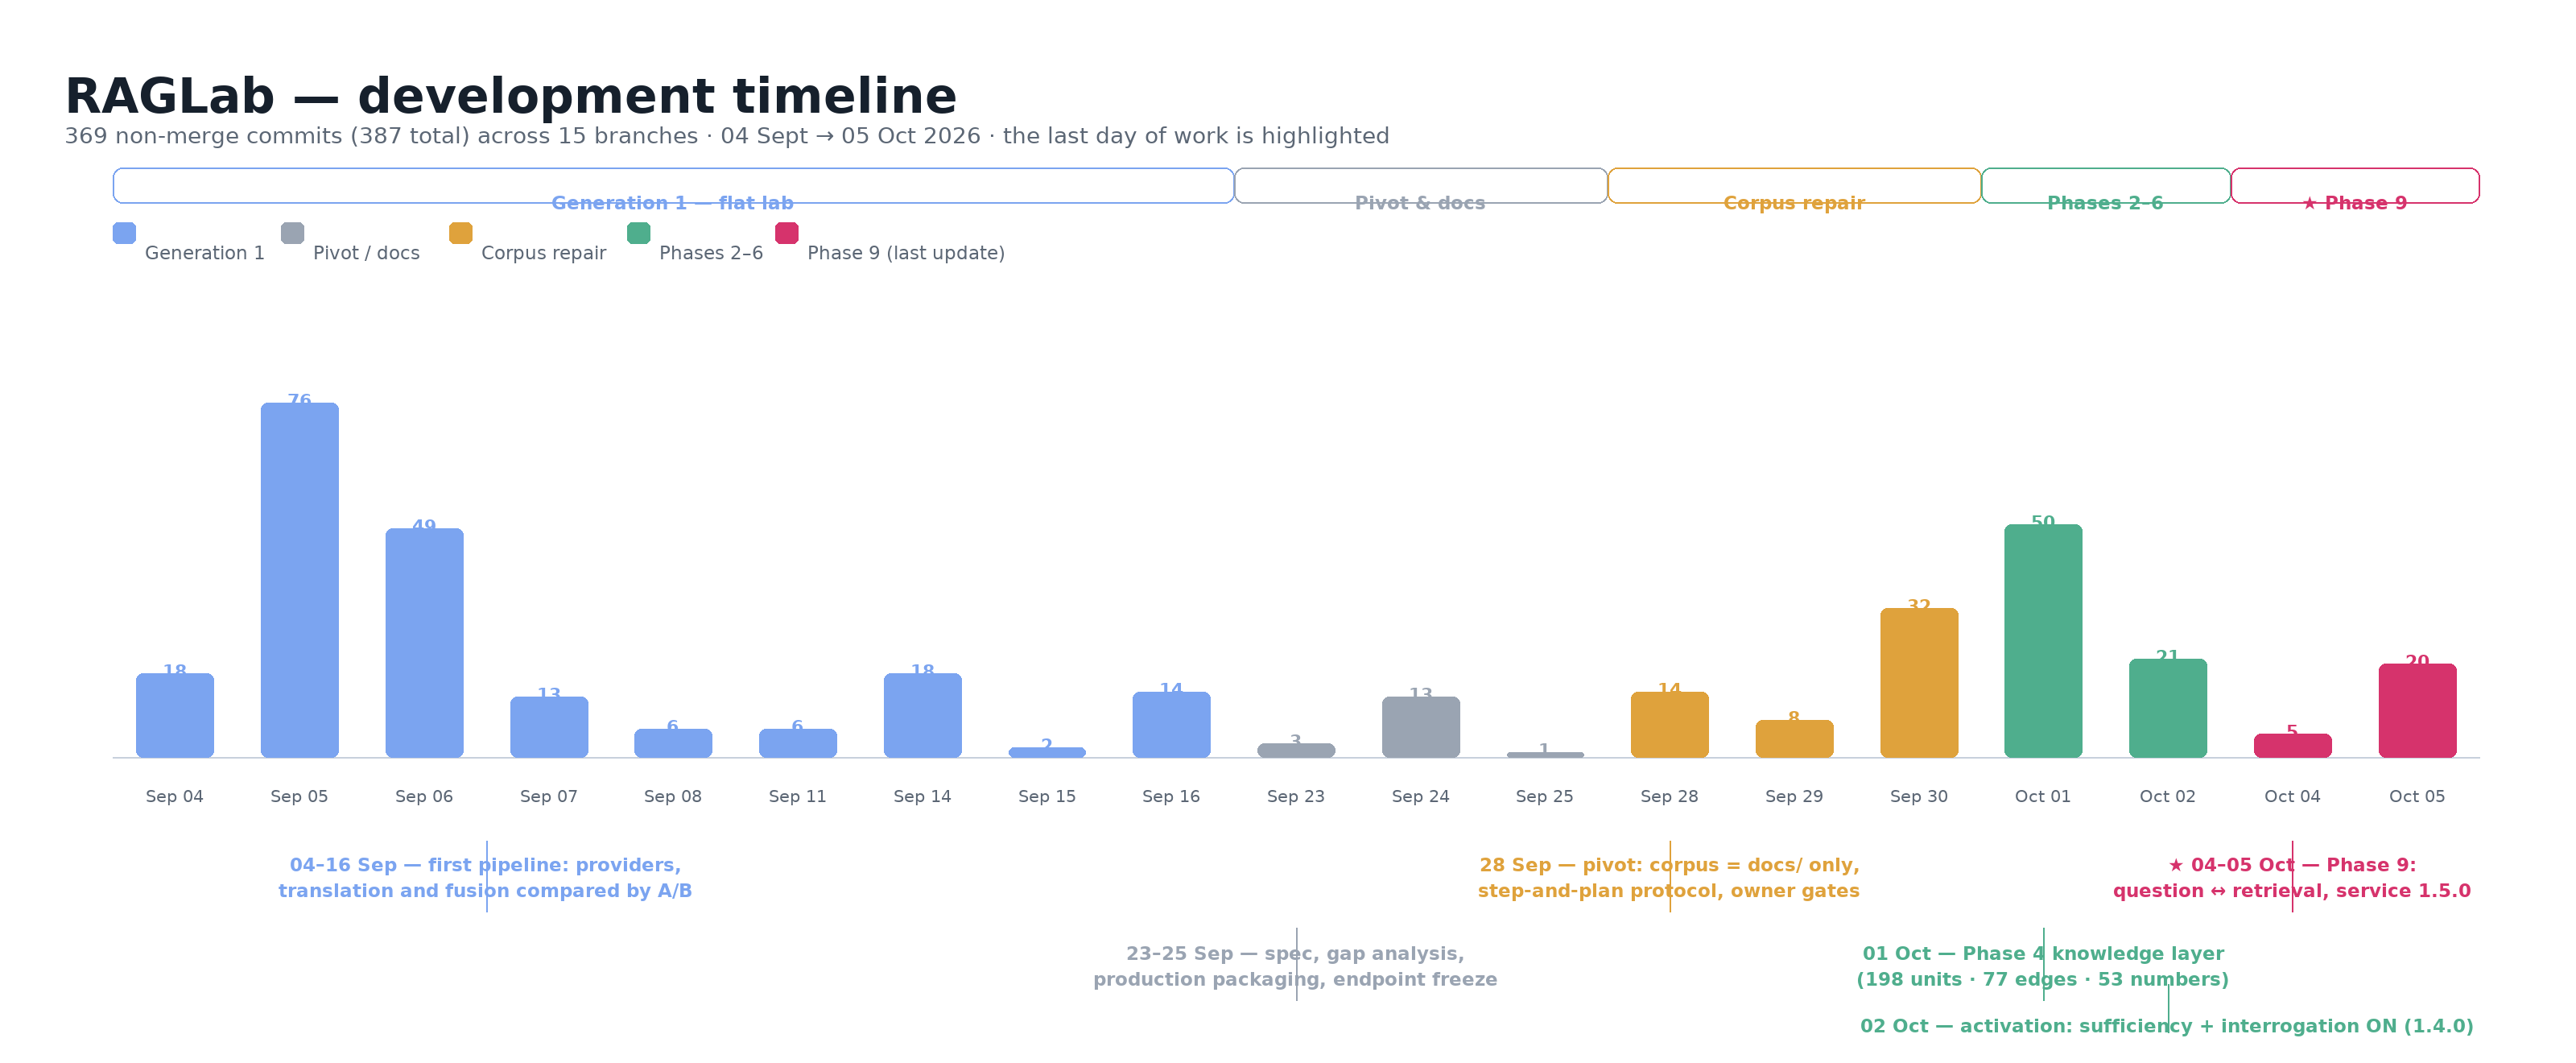
\includegraphics[width=\textwidth]{timeline.png}
\caption{Chronologie du développement : 369 commits répartis sur 19 journées de travail, la dernière
journée (04--05 octobre) mise en évidence.}
\end{figure}

L'architecture a \textbf{changé en profondeur au milieu du projet} :

\begin{center}
\begin{tabular}{p{4.3cm}p{10.2cm}}
\toprule
\textbf{Période} & \textbf{Architecture} \\
\midrule
\textcolor{genone}{04 $\rightarrow$ 23 sept.} & Génération 1 — pipeline plat, multi-fournisseurs,
traduction, fusion explorée par A/B \\
\textcolor{genpivot}{24 $\rightarrow$ 28 sept.} & Pivot — rapport cible, analyse d'écart,
refondation sur \texttt{docs/}, réparation du corpus \\
\textcolor{gentwo}{24 sept. $\rightarrow$ 05 oct.} & Génération 2 — quatre couches gouvernées :
structure, connaissance, compréhension, livraison \\
\textcolor{genlast}{\textbf{04--05 oct. (dernière évolution)}} & \textbf{Phase 9 — lien
question $\leftrightarrow$ corpus, service 1.5.0} \\
\bottomrule
\end{tabular}
\end{center}

Le moteur commun aux deux générations est inchangé et volontairement figé : vectorisation NVIDIA,
index local en cosinus, génération par le modèle épinglé, contrôle des citations. Ce qui a changé,
c'est \textbf{ce qui entoure} ce moteur : la nature du corpus, la manière de découper, et surtout
l'ajout de couches explicites de connaissance, de compréhension et de traçabilité.

\section{Génération 1 — le laboratoire de recherche d'information}
La première génération est un pipeline linéaire, orienté comparaison : corpus de test (fictif puis
compilé depuis le web) ; découpage \texttt{size} par défaut, cartes de découpage revues
manuellement, puis mode \texttt{restructure} ; vectorisation multi-fournisseurs avec validation
stricte et mise en cache ; indexation ChromaDB avec empreinte de découpage ; recherche
\texttt{vector}, \texttt{rrf}, \texttt{blend} et politiques de départage ; variantes de requête par
traduction automatique puis fusion des variantes ; réponse multi-fournisseurs avec chaîne de repli,
contrat JSON \texttt{grounded-v1} et contrôle des citations.

\textbf{Pourquoi elle a été remplacée.} Cette génération répondait à une question de mesure
(« quel découpage, quel modèle, quelle fusion gagne ? ») mais pas à la question apparue avec le
rapport cible : « le système peut-il \emph{décider} — citer, douter, refuser, tracer ? » Aucun
réglage de recherche ne produit une notion de suffisance, des unités de connaissance stables ou un
journal d'audit.

\section{Le pivot (24 $\rightarrow$ 28 septembre 2026)}
\begin{enumerate}
  \item \textbf{Spécification inversée.} Un document de spécification technique a été produit par
        investigation statique du code : chaque affirmation y est citée (fichier, symbole, ligne)
        et étiquetée \emph{observé}, \emph{déduit} ou \emph{inconnu}.
  \item \textbf{Analyse d'écart.} Le rapport cible a été confronté à cette spécification : le
        système était \emph{en avance} sur certaines hypothèses (contrôle des citations, taxonomie
        de refus, refus de servir un index périmé) et \emph{en retard} sur d'autres (intention,
        plan de preuve, suffisance, gouvernance documentaire, journal d'audit, identifiants
        d'unité stables).
  \item \textbf{Refondation sur le corpus réel.} Le corpus de travail est constitué uniquement des
        quatre documents réels ; la campagne compilée depuis le web est retirée. Le protocole
        « étape et plan » est adopté à cette date.
  \item \textbf{Réparation du corpus.} Les quatre documents ont été corrigés par voie linguistique
        uniquement : 215 corrections pour la loi (29 lots), 35 pour la circulaire (dont les
        28 nombres corrompus), 23 pour le guide (numérotation hiérarchique inversée) et 21 pour le
        support de formation. Chaque journal est vérifié automatiquement et chaque document adopté
        par le donneur d'ordre. Le corpus d'évaluation compte dès lors \textbf{339 fragments}.
\end{enumerate}

\section{Génération 2 — l'architecture en couches}

\subsection{Couche 1 — corpus et structure}
\begin{table}[H]
\centering
\small
\begin{tabular}{p{3.0cm}p{11.5cm}}
\toprule
\textbf{Module} & \textbf{Rôle} \\
\midrule
\texttt{loader.py} & Lecture PDF/DOCX/MD, normalisation arabe (NFKC, formes de présentation,
unification des alif, suppression du tatweel et des diacritiques), détection de langue \\
\texttt{restructure.py} & Découpage structurel en trois étapes ; réparation de l'ordre visuel par
reconstruction de zones ; adoption des textes corrigés \\
\texttt{chunker.py} & Découpage historique \texttt{size} (220/40) ; empreinte de découpage
(version 4) encodant mode, taille, recouvrement et tokenizer \\
\texttt{docstore.py} & Documents poussés par l'application, versionnés par empreinte SHA-256 ;
index marqué « périmé » jusqu'à la prochaine indexation \\
\texttt{store.py} & ChromaDB local (cosinus), index lexical BM25, fusion RRF/blend, refus de
servir un index incohérent, purge par source \\
\bottomrule
\end{tabular}
\end{table}

Deux garde-fous structurent cette couche : \textbf{l'index est auto-descriptif} (chaque fragment
porte l'empreinte du découpage et de l'espace vectoriel ; une recherche sur un index périmé est
refusée avec la marche à suivre) et un \textbf{verrou d'indexation} (pendant une indexation, toutes
les lectures d'index renvoient un conflit explicite plutôt qu'une lecture incohérente).

\subsection{Couche 2 — la couche de connaissance}
Construite sur la loi 2016-48 (document choisi par le donneur d'ordre), cette couche est
\textbf{déterministe et déclarative} : les données sont des fichiers versionnés, validés par des
contrôles automatiques et révisables ligne à ligne.

\begin{table}[H]
\centering
\small
\begin{tabular}{p{3.4cm}p{7.4cm}p{3.7cm}}
\toprule
\textbf{Élément} & \textbf{Contenu} & \textbf{Contrôle} \\
\midrule
Unités de connaissance & 198 unités (= les 198 articles), texte littéral, identifiant stable
\texttt{loi-2016-48:artNNN}, chemin hiérarchique, type fonctionnel gouverné & Couverture 198/198,
littéralité, stabilité des identifiants \\
Relations & 77 références internes + 1 relation d'ancrage (circulaire $\rightarrow$ article 11) &
Preuve littérale obligatoire, cibles existantes \\
Chiffres structurés & 53 enregistrements (14 taux, 28 délais, 5 plafonds, 6 sanctions) + table de
corrections (15 lignes), servis par \texttt{GET /numbers} & Chaque valeur présente littéralement
dans son unité \\
Gouvernance & 6 axes (autorité, vigueur, portée, public, domaine, source) dans les métadonnées des
fragments & Cohérence registre $\leftrightarrow$ corpus \\
Index d'unités & 198 lignes descriptives indexées dans une collection isolée & Mesuré :
100/100/100 contre 67/92/92 (§4.6) \\
\bottomrule
\end{tabular}
\end{table}

L'ajout de \texttt{GET /numbers} est significatif : c'est la \textbf{première extension
autorisée} sous le gel des points d'entrée, conçue comme strictement additive — lecture seule,
filtrable, fonctionnant même sur un index vide, sans modifier aucun point d'entrée existant.

\subsection{Couche 3 — la compréhension de la demande}
Sa règle fondatrice : \textbf{déterministe d'abord, modèle ensuite, et jamais deux fois}.

\begin{table}[H]
\centering
\small
\begin{tabular}{p{4.3cm}p{7.7cm}p{2.5cm}}
\toprule
\textbf{Module} & \textbf{Fonction} & \textbf{État} \\
\midrule
\texttt{intent.py} & Classification de l'intention par règles déclarées ; découpage des demandes
composées ; détection d'ambiguïté influente & Actif \\
\texttt{evidence\_plan.py} & Dérive de l'intention les \textbf{exigences de preuve} — jamais la
réponse & Actif \\
\texttt{sufficiency.py} & Confronte plan et fragments récupérés ; état de suffisance ;
contradictions ; tours de recherche guidés bornés & Actif \\
\texttt{decompose.py} & Décompose chaque question en micro-questions à exigence unique & Construit,
non câblé \\
\texttt{interrogate.py}, \texttt{topic\_map.py} & Si (et seulement si) rien n'est couvert : un
appel borné transforme la demande pratique en question technique & \textbf{Actif par défaut} \\
\texttt{relational\_expansion.py} & Élargit la recherche le long des relations, en queue de liste &
Désactivé (mesuré neutre) \\
\texttt{micro\_retrieval.py} & Recherche par micro-question + fusion & Désactivé (mesuré
défavorable) \\
\bottomrule
\end{tabular}
\end{table}

Les garanties de l'interrogation expliquent son acceptation : \textbf{échec fermé} (sortie mal
formée, sujet inventé, exigence inventée ou reformulation identique $\Rightarrow$ refus normal),
\textbf{divulgation complète} (champs \texttt{understood\_as}, \texttt{original\_question} et
\texttt{interrogation}) et \textbf{coût visible} (durée de l'appel exposée séparément).

\subsection{Couche 4 — livraison et audit}
\begin{itemize}
  \item \textbf{Invite de génération} (\texttt{grounded-v1}) : question et extraits déclarés comme
        données non fiables ; sortie JSON stricte (affirmations + preuves), sans prose libre.
  \item \textbf{Contrôle des citations} : appartenance des citations, contrôle numérique, contrôle
        de politique. Les fragments de loi cités portent l'identifiant d'unité stable, permettant
        de citer un article de manière durable.
  \item \textbf{Engagement de suffisance} : si rien n'est couvert, le service refuse \textbf{avant}
        tout appel de génération, avec une référence nommant les exigences manquantes ; si la
        couverture est partielle, une seule régénération bornée est autorisée.
  \item \textbf{Assainissement} : les données personnelles reconnaissables (courriel, téléphone,
        RIB/IBAN tunisien, CIN) sont remplacées par des étiquettes \textbf{après} le contrôle.
  \item \textbf{Journal d'audit} : chaque requête laisse une trace JSONL (identifiant, horodatage,
        question assainie, statut, état de suffisance, modèle, compteurs, latence), exposée par
        \texttt{GET /audit} avec rétention bornée.
\end{itemize}

\subsection{Le cycle d'une requête}
\begin{verbatim}
Question (ar / fr / en)
  -> authentification, court-circuit de salutation, verrou d'indexation
  -> intention -> plan de preuve
  -> recherche dense sur la question ORIGINALE (jamais traduite), top 5
  -> suffisance sur les fragments recuperes
       |- suffisant  -> generation directe (zero appel supplementaire)
       |- partiel    -> une seule regeneration bornee sur les points couverts
       '- rien       -> UN appel d'interrogation borne -> nouvelle recherche -> meme controle
  -> construction du contexte (budget 3000 tokens ; un extrait tronque est ecarte)
  -> generation JSON ancree -> controle des citations -> assainissement -> journal
  -> reponse citee, ou refus motive (les deux sont des reponses valides)
\end{verbatim}

\subsection{Portes et valeurs par défaut}
Toutes les briques expérimentales sont placées derrière des \textbf{portes} explicites. Portes
activées : champs de suffisance, engagement de suffisance, interrogation, vocabulaire de concepts
et ponts entre systèmes d'écriture. Portes désactivées par la mesure : expansion relationnelle,
recherche par micro-question. Chaque porte désactivée restaure le comportement antérieur
\textbf{octet pour octet}, ce qui est vérifié par un test dédié.

\section{Le service et les interfaces}
\begin{table}[H]
\centering
\small
\begin{tabular}{p{3.4cm}p{11.1cm}}
\toprule
\textbf{Aspect} & \textbf{Mise en œuvre} \\
\midrule
Points d'entrée & 27 routes : santé, profil et modèles, clés, inspection, fragments, indexation,
recherche, réponse, évaluation, documents, diagnostics, audit, chiffres \\
Version & \texttt{SERVICE\_VERSION = 1.5.0}, incrémentée à chaque changement de service \\
Contrat & Document de contrat humain + schéma OpenAPI généré \\
Authentification & Jeton partagé (\texttt{X-Service-Token}), comparaison à temps constant ; service
prévu derrière la passerelle applicative \\
Erreurs & Enveloppe unique \texttt{\{"detail": \{"reason": ...\}\}}, raisons stables, valeurs
sensibles filtrées \\
Gel & Aucun point d'entrée existant ne change ; évolutions additives \\
Intégration & CLI, console locale, console HTTP (banc d'essai d'intégration de l'application) \\
\bottomrule
\end{tabular}
\end{table}

Le service est livré avec un \texttt{Dockerfile} et un \texttt{docker-compose.yml} (volumes pour
l'index, le cache de vectorisation et les documents poussés), et son intégration est documentée
pour l'équipe applicative : contrat HTTP, guide de requêtes exactes, maquette d'interface et guide
de déploiement.

\section{\textcolor{genlast}{$\bigstar$ La dernière évolution (Phase 9, 05 octobre 2026)}}
C'est l'état \textbf{actuel} du système : les sections précédentes décrivent la trajectoire,
celle-ci décrit le point d'arrivée.

\paragraph{Le problème visé.} La carte des sujets utilisée par l'interrogation était dérivée des
seuls titres de sections ; elle contenait des entrées sans substance et ne garantissait pas que le
sujet choisi corresponde au corpus réellement interrogeable.

\paragraph{Ce qui a changé.}
\begin{enumerate}
  \item \textbf{Carte de sujets reconstruite} — 262 nœuds adossés aux sources (198 unités de loi +
        20 chapitres de la circulaire), chacun avec identifiant, chemin et extrait ; l'interrogation
        reçoit des identifiants à correspondance exacte. Service en version 1.5.0, sans modifier la
        forme des réponses.
  \item \textbf{Mesures dédiées} — recherche seule sur sept cas porteurs de preuve (hit@1/3/5 = 5/7
        en mode dense) ; comparaison en direct de la carte des sujets (12 appels, tous correctement
        analysés, 4/5 $\rightarrow$ 5/5 de sujets cibles atteints) ; sondage de bout en bout sur
        \texttt{POST /answer} : 3 réponses ancrées, 3 refus, toutes les réponses générées validées,
        zéro erreur de fournisseur. L'augmentation du nombre de fragments récupérés (5, 12, 20) ne
        change aucun résultat.
  \item \textbf{Corrections issues de l'exploitation réelle} :
    \begin{itemize}
      \item le tour guidé \textbf{ne s'exécutait jamais dans le service déployé} — l'appel au
            contrôle de suffisance y était fait sans fonction de recherche ; le défaut
            n'apparaissait que sur le service réel ;
      \item \textbf{cause racine d'une erreur d'intention en français} — le motif
            \texttt{Quelle} s'appliquait à l'intérieur du mot \texttt{Quelles}, classant une
            question procédurale comme définitionnelle ; les marqueurs procéduraux français ont été
            ajoutés et ancrés ;
      \item \textbf{doublons d'indexation bloqués} — une poussée identique à un document du corpus
            est refusée par empreinte SHA-256 (et non par nom), ce qui a mis fin à un gonflement de
            l'index (859 fragments dupliqués constatés) ;
      \item \textbf{divulgation des réponses réorientées} — un vocabulaire de concepts (8 lignes
            familier $\rightarrow$ terme du corpus) et deux champs additifs signalent qu'une
            réponse a été produite après réinterprétation de la demande.
    \end{itemize}
  \item \textbf{État vérifié} — porte hors ligne verte (463 tests unitaires + 121 contrôles),
        intégration continue verte (suite hors ligne + construction et import de l'image conteneur),
        jeux de questions et index de production inchangés.
\end{enumerate}

\paragraph{Ce qui reste ouvert} (et n'est engagé par aucun défaut) : métadonnées topiques au niveau
des fragments (\texttt{path}, \texttt{level}, \texttt{parent\_id}), bras de recherche topique et
leur mesure, facettes de vocabulaire, campagne de mesure finale.

\section{Ingénierie de la qualité}
\begin{table}[H]
\centering
\small
\begin{tabular}{p{3.4cm}p{11.1cm}}
\toprule
\textbf{Dispositif} & \textbf{Contenu} \\
\midrule
Tests hors ligne & 463 tests unitaires + 121 contrôles déterministes + compilation + inspection +
vérification des dépendances \\
Intégration continue & 7 scénarios : porte principale à chaque poussée, suite « modèles réels » sur
déclenchement manuel (coût maîtrisé), harnais lourd, catalogues, juge de recherche, A/B de réponses,
tests réels par étiquette \\
Portes de qualité & Empreintes d'index, refus de service pendant l'indexation, absence de repli,
refus avant génération, échec fermé de l'interrogation \\
Reproductibilité & Caches adressés par empreinte ; exécutions archivées ; chiffres rattachés à un
commit et à un identifiant d'exécution \\
Documentation & Contrat, guide de requêtes, maquette d'interface, guide de déploiement, contrat de
travail pour les sessions suivantes \\
\bottomrule
\end{tabular}
\end{table}

% ====================== CHAPITRE 4 ======================
\chapter{Évaluation, résultats et limites}

\section{Corpus et jeux de questions}
Le corpus d'évaluation est celui décrit au §3.3 : quatre documents réels, réparés puis adoptés,
soit \textbf{339 fragments} sur le bras structurel (le découpage réellement obtenu en intégration
continue, avec le tokenizer complet, en produit 858 ; c'est cette différence, propre au tokenizer,
qui explique que certains contrôles soient exprimés en parts et non en nombres absolus).

\begin{table}[H]
\centering
\small
\begin{tabular}{p{3.6cm}p{3.0cm}p{7.9cm}}
\toprule
\textbf{Jeu} & \textbf{Taille} & \textbf{Composition} \\
\midrule
\texttt{questions\_50.json} & 50 cas (45 évaluables + 5 hors périmètre) & 10 verbatim,
20 paraphrases, 15 transfrontaliers (6 fr, 9 en) ; 32 ar / 8 fr / 10 en \\
\texttt{questions\_targets.json} & 10 cas arabes & 2 par catégorie : familier, synonymes,
implicite, composé, ambigu \\
\bottomrule
\end{tabular}
\end{table}

Chaque sous-chaîne attendue a été vérifiée automatiquement : présence littérale dans le document
attendu \textbf{et} caractère distinctif dans le corpus (les concepts partagés entre documents,
comme la murabaha, portent une preuve propre à chaque document). La répartition par document est de
12 cas pour la loi, 10 pour la circulaire, 11 pour le guide et 12 pour le support de formation.

\section{Protocole de mesure}
\begin{itemize}
  \item \textbf{Comparaison appariée} : les deux bras comparés sont mesurés dans la même exécution.
  \item \textbf{Tolérance} : $\pm 2$ points pour toute comparaison inter-exécutions.
  \item \textbf{Deux étages} : un étage hors ligne (BM25 seul, déterministe, gratuit) qui sert de
        filtre rapide, et un étage \emph{live} (vectorisation et modèles réels) qui tranche.
  \item \textbf{Comportement final} : au-delà de hit@$k$, on mesure le statut (réponse ancrée /
        refus) et la conformité des citations.
\end{itemize}

\section{Découpage : fenêtre fixe contre structurel}
Mesure hors ligne (BM25 seul, $k = 20$), sur le jeu de 50 cas :

\begin{table}[H]
\centering
\begin{tabular}{lccc}
\toprule
\textbf{Bras} & \textbf{hit@1} & \textbf{hit@3} & \textbf{hit@5} \\
\midrule
\texttt{size} 220/40 & 42 & 60 & 62 \\
\texttt{restructure} (corpus réparé adopté) & \textbf{62} & \textbf{82} & \textbf{87} \\
\bottomrule
\end{tabular}
\end{table}

Par langue : arabe 43/57/60 $\rightarrow$ 67/87/93 ; anglais 44/89/89 $\rightarrow$ 67/100/100 ;
français inchangé (33/33/33), plafond lexical que seul l'étage vectoriel pouvait franchir.

Mesure \textbf{live} (vectorisation et modèles réels, même jeu) :

\begin{table}[H]
\centering
\begin{tabular}{lccc}
\toprule
\textbf{Bras} & \textbf{hit@1} & \textbf{hit@3} & \textbf{hit@5} \\
\midrule
\texttt{size} & 51 & 64 & 71 \\
\texttt{restructure} & \textbf{71} & \textbf{80} & \textbf{87} \\
\bottomrule
\end{tabular}
\end{table}

Le gain est net et reproductible : \textbf{+20 points de hit@1}. Les cas manqués par le bras
vectoriel sont, de façon complémentaire, retrouvés par le bras lexical — observation qui a motivé
l'essai d'un réordonnanceur déterministe, activé par défaut après mesure.

\section{Modes de recherche : la fusion ne paie pas}
\begin{table}[H]
\centering
\small
\begin{tabular}{lcccl}
\toprule
\textbf{Mode} & \textbf{hit@1} & \textbf{hit@3} & \textbf{hit@5} & \textbf{Lecture} \\
\midrule
\texttt{vector} & \textbf{71} & 80 & \textbf{87} & retenu par défaut \\
\texttt{rrf} (BM25 fusionné) & 71 & 80 & 82 & égal en tête, en retrait en rappel \\
\texttt{blend} ($\lambda = 0{,}7$) & 62 & 80 & 84 & en retrait en tête \\
\bottomrule
\end{tabular}
\end{table}

En français, l'écart est plus marqué : le mode dense obtient 50/67/67, contre 33/33/50 pour RRF et
33/33/67 pour le blend. La règle de décision retenue (« ne changer de défaut que si le nouveau mode
gagne \emph{sans} régression sur les cas verbatim et hors périmètre ») conduit à conserver le mode
dense, les deux autres restant des options explicites et la décision révisable.

\section{Indépendance du modèle de réponse}
\begin{table}[H]
\centering
\small
\begin{tabular}{lcccc}
\toprule
\textbf{Modèle} & \textbf{Réponses} & \textbf{Refus} & \textbf{Erreurs} & \textbf{Refus par la porte} \\
\midrule
\texttt{qwen/qwen3.8-max:free} (retenu) & 37 & 13 & 0 & 7 \\
\texttt{moonshotai/kimi-k3} & 27 & 14 & 9 & 7 \\
\bottomrule
\end{tabular}
\end{table}

Accord de statut entre les deux modèles : \textbf{0,720}. Surtout, lorsque les deux modèles
répondent, les sources citées sont \textbf{identiques} (similarité de Jaccard = 1,000) : à contexte
fixé, la divergence entre modèles porte sur l'acceptation ou le refus, pas sur les citations. Ce
résultat conforte un choix d'architecture — la recherche est indépendante du modèle de réponse,
puisque le modèle ne voit jamais la question sous forme de requête — et déplace le travail restant
vers la complétude des preuves.

\section{La couche de connaissance}
\textbf{Index d'unités} — les 198 lignes descriptives des articles, indexées dans une collection
isolée et jugées par la même règle de comparaison, sur les 12 questions portant sur la loi :

\begin{table}[H]
\centering
\begin{tabular}{lccc}
\toprule
\textbf{Bras} & \textbf{hit@1} & \textbf{hit@3} & \textbf{hit@5} \\
\midrule
Référence (découpage structurel) & 67 & 92 & 92 \\
Index d'unités & \textbf{100} & \textbf{100} & \textbf{100} \\
\bottomrule
\end{tabular}
\end{table}

Chaque question de loi, y compris les questions transfrontalières, trouve son article au rang 1 sur
la surface descriptive.

\textbf{Catégories cibles} — mesure live du jeu de 10 cas arabes :

\begin{table}[H]
\centering
\small
\begin{tabular}{lccc}
\toprule
\textbf{Catégorie} & \textbf{hit@1} & \textbf{hit@3} & \textbf{hit@5} \\
\midrule
Demande composée & 100 & 100 & 100 \\
Implicite et ambiguë & 50 & 100 & 100 \\
Synonymes & 50 & 50 & 50 \\
Langage familier & 0 & 0 & 0 \\
\bottomrule
\end{tabular}
\end{table}

L'activation d'un lexique institutionnel de 16 entrées n'apporte \textbf{rien} sur le bras
vectoriel, alors qu'il améliorait le bras lexical : ce résultat a conduit à laisser le lexique
désactivé, décision documentée et révisable.

\section{\textcolor{genlast}{$\bigstar$ La dernière campagne (Phase 9)}}
\begin{table}[H]
\centering
\small
\begin{tabular}{p{6.2cm}p{8.3cm}}
\toprule
\textbf{Mesure} & \textbf{Résultat} \\
\midrule
Recherche seule, 7 cas porteurs de preuve & hit@1/3/5 = 5/7 (mode dense) \\
Comparaison de la carte des sujets, 12 appels réels & 12/12 analysés sans erreur ; sujets cibles
atteints 4/5 $\rightarrow$ \textbf{5/5} \\
Sondage de bout en bout, 6 questions inchangées & \textbf{3 réponses ancrées / 3 refus}, toutes les
réponses générées validées, 0 erreur fournisseur \\
Effet du nombre de fragments (5, 12, 20) & aucun changement de résultat \\
Défaut découvert et corrigé & le tour guidé ne s'exécutait pas dans le service déployé \\
Cause racine corrigée & \texttt{Quelle} reconnu à l'intérieur de \texttt{Quelles} \\
Doublons & poussée identique refusée par SHA-256 (859 fragments dupliqués constatés) \\
État final & porte verte : 463 tests + 121 contrôles ; CI verte ; jeux et index inchangés \\
\bottomrule
\end{tabular}
\end{table}

Leçon méthodologique : \textbf{les trois défauts les plus coûteux n'ont été trouvés que par une
exécution réelle}, jamais par la suite de tests — un banc de test ne mesure que ce qu'il simule.
C'est ce qui justifie la règle adoptée en fin de stage : toute affirmation portant sur le service
déployé doit être vérifiée sur le service déployé.

\section{Robustesse}
Six scénarios adversariaux sont vérifiés automatiquement contre le contrôle des citations :
citation fabriquée, citation empruntée à une autre source, nombre calculé, identifiant de citation
inconnu, marqueur de citation dans le texte de l'affirmation, et injection d'instruction dans la
question ou dans un extrait. Tous sont refusés par le contrôle déterministe. Une limite est
assumée : le contrôle garantit que les mots et les nombres proviennent bien de la source, \textbf{pas}
que l'affirmation en découle logiquement.

D'autres défauts d'exploitation ont été corrigés en cours de stage, chacun sanctionné par un test de
régression : fuite d'erreur réseau en erreur 500 (désormais 502 explicite), verrou d'indexation
pendant l'ingestion, nommage de fichier malveillant, priorité des variables d'environnement dans la
composition conteneur (un jeton codé en dur écrasait silencieusement la configuration — incident
réel chez l'équipe plateforme, corrigé et documenté).

\section{Limites}
\begin{table}[H]
\centering
\small
\begin{tabular}{p{4.7cm}p{9.8cm}}
\toprule
\textbf{Limite} & \textbf{Portée} \\
\midrule
Contrôle des citations $\neq$ implication & Une phrase correctement sourcée peut rester une
interprétation abusive \\
Aucun seuil de similarité & Les 5 extraits sont transmis même s'ils sont hors sujet ; la sécurité
repose sur la suffisance et le refus \\
Processus unique & Un profil, un index, une indexation à la fois ; pas de montée en charge
horizontale \\
Mise à jour par réindexation & Un document remplacé continue de servir ses anciens fragments \\
Tokenizer & Sans le fichier de vocabulaire \texttt{cl100k}, une estimation remplace le compte réel ;
seule la CI fait foi \\
Détection de langue heuristique & Des erreurs d'étiquetage restent possibles \\
Pas de mémoire conversationnelle ni de flux & Choix assumés de la configuration actuelle \\
Jeux de tests restreints et corrélés & 50 + 10 cas ne constituent ni une garantie de sécurité, ni
une garantie juridique \\
\bottomrule
\end{tabular}
\end{table}

Le dépôt porte lui-même la mention explicite : \textbf{le système n'est pas prêt pour une mise en
production bancaire} ; il est adapté à un pilote supervisé sur des documents approuvés et non
confidentiels.

\section{Coûts et exploitation}
Le recours à des modèles gratuits et la mise en cache adressée par empreinte maintiennent le coût
d'exploitation à un niveau quasi nul pour les campagnes hors ligne. Les campagnes \emph{live} sont
déclenchées manuellement et bornées ; chaque campagne publie ses chiffres dans une annotation de
l'exécution, ce qui permet de comparer sans télécharger d'artefacts. La conteneurisation (image,
volumes, sondage de santé tenant compte du jeton) et un guide de déploiement ont été livrés à
l'équipe plateforme en fin de stage.

% ====================== CONCLUSION ======================
\chapter*{Conclusion générale et perspectives}
\addcontentsline{toc}{chapter}{Conclusion générale et perspectives}

\section*{Bilan}
Le stage a produit un système de question-réponse documentaire complet, mesuré et documenté,
aujourd'hui en état de fonctionner sur un corpus bancaire réel en arabe :

\begin{itemize}
  \item \textbf{une chaîne complète} — lecture et réparation des documents, découpage structurel,
        vectorisation, index local, recherche dense et lexicale, génération ancrée, contrôle des
        citations, refus motivé ;
  \item \textbf{une architecture en couches} — structure, connaissance, compréhension, livraison —
        dont la dernière génération est née d'un changement d'architecture assumé en milieu de
        projet ;
  \item \textbf{des résultats mesurés} — +20 points de hit@1 par le découpage structurel
        (51 $\rightarrow$ 71), index d'unités à 100/100/100, accord inter-modèles de 0,720 avec
        citations identiques, jeux gelés comme référence de non-régression ;
  \item \textbf{un service} — 27 points d'entrée, contrat gelé et versionné, journal d'audit,
        assainissement des données personnelles, image conteneur et guide de déploiement.
\end{itemize}

\section*{Enseignements}
\begin{enumerate}
  \item \textbf{La mesure remplace l'opinion.} Chaque choix structurant (découpage structurel,
        recherche dense, lexique désactivé, expansion relationnelle abandonnée) a été tranché par
        des chiffres appariés, et plusieurs intuitions raisonnables ont été rejetées par les
        données.
  \item \textbf{La gouvernance des décisions fait partie de l'architecture.} Le protocole
        « étape et plan », les portes d'activation et les jeux gelés ont permis de reprendre un
        projet interrompu plusieurs fois sans régression silencieuse.
  \item \textbf{Le réel est le seul juge.} Les défauts les plus graves — tour guidé inerte dans le
        service, classification d'intention erronée en français, doublons d'indexation — étaient
        invisibles en test et évidents en exploitation.
\end{enumerate}

\section*{Perspectives}
\begin{enumerate}
  \item \textbf{Décision d'identité et de rôles} (phase 7, en attente) : conditionne tout usage
        au-delà d'un pilote interne.
  \item \textbf{Métadonnées topiques au niveau des fragments} (\texttt{path}, \texttt{level},
        \texttt{parent\_id}) : suite identifiée de la Phase 9, à construire dans une collection
        isolée avant toute réindexation de production.
  \item \textbf{Bras de recherche topique et facettes} : mesurer, sur les mêmes jeux gelés, la
        recherche par facettes et sa fusion avec le mode dense.
  \item \textbf{Campagne de clôture} : re-mesurer tous les bras, documenter les régressions, puis
        décider des valeurs par défaut.
  \item \textbf{Industrialisation} : multi-utilisateurs, mise à jour incrémentale, observabilité
        et évaluation adversariale continue.
\end{enumerate}

% ====================== ANNEXES ======================
\appendix
\chapter{Glossaire}
\begin{table}[H]
\centering
\small
\begin{tabular}{p{3.0cm}p{3.0cm}p{8.5cm}}
\toprule
\textbf{Terme} & \textbf{Translittération} & \textbf{Sens} \\
\midrule
--- & \emph{al-murabaha} & Vente à prix de revient majoré d'une marge connue \\
--- & \emph{al-sigha} & Forme contractuelle (offre et acceptation) \\
--- & \emph{al-fasl} & Article (dans la loi) / chapitre (dans la circulaire) \\
--- & \emph{nafidh} & En vigueur \\
--- & \emph{kafin} & Suffisant (état de suffisance) \\
--- & \emph{ghayr kafin} & Insuffisant \\
--- & \emph{mutaarid} & Contradictoire (deux sources en désaccord) \\
RAG & --- & \emph{Retrieval-Augmented Generation} \\
hit@$k$ & --- & Le document/extrait attendu figure-t-il parmi les $k$ premiers résultats \\
RRF & --- & \emph{Reciprocal Rank Fusion} : fusion par rang réciproque \\
BM25 & --- & Fonction de classement lexical classique en recherche d'information \\
Citation gate & --- & Contrôle déterministe d'appartenance des citations et des nombres \\
Suffisance & --- & Confrontation du besoin de preuve au contenu réellement récupéré \\
Porte (\emph{gate}) & --- & Interrupteur d'activation d'une brique, avec repli vérifié \\
\bottomrule
\end{tabular}
\end{table}

\emph{Note : les termes arabes figurent en écriture arabe dans la version Markdown du rapport et
dans le PDF joint ; ils sont translittérés ici pour que ce fichier compile avec pdflatex sans
police arabe.}

\chapter{Provenance des chiffres}
\begin{table}[H]
\centering
\small
\begin{tabular}{p{5.6cm}p{9.0cm}}
\toprule
\textbf{Chiffre} & \textbf{Source dans le dépôt} \\
\midrule
387 commits, 15 branches, une trentaine d'étiquettes & Historique Git du dépôt \\
220 fichiers, 39\,491 lignes de Python & Inventaire du dépôt à l'état final \\
4 documents, 339 fragments, réparations 215/35/23/21 & \texttt{audits/MASTER\_INDEX.md},
\texttt{AGENTS.md} \\
50 questions (10/20/15/5) et 10 cas cibles & \texttt{audits/QUESTIONS\_MATRIX.md},
\texttt{audits/PHASE3\_INTERVENTIONS.md} \\
BM25 42/60/62 $\rightarrow$ 62/82/87 ; live 51/64/71 $\rightarrow$ 71/80/87 &
\texttt{audits/PHASE2\_BASELINES.md} (exécutions 3.1 et 3.2) \\
vector 71/80/87 · rrf 71/80/82 · blend 62/80/84 & Idem (exécution 3.2) \\
Accord 0,720 ; Jaccard 1,000 & Idem (exécution 3.3) \\
Index d'unités 100/100/100 vs 67/92/92 & \texttt{audits/PHASE4\_KNOWLEDGE.md} \\
198 unités, 77 relations, 53 chiffres, 6 axes & Idem \\
Catégories cibles 50/70/70 & \texttt{audits/PHASE3\_INTERVENTIONS.md} \\
Phase 9 : 5/7, 4/5 $\rightarrow$ 5/5, 3 réponses / 3 refus &
\texttt{audits/PHASE9\_STRUCTURE/} \\
463 tests + 121 contrôles ; CI verte & Message de commit final et intégration continue \\
27 routes, version 1.5.0 & \texttt{service.py}, \texttt{CONTRACT.md} \\
\bottomrule
\end{tabular}
\end{table}

\chapter{Reproduction}
\begin{verbatim}
# Environnement
cd <depot>/raglab
python3 -m venv .venv && source .venv/bin/activate
pip install -r requirements.txt

# Porte hors ligne complete (aucun appel de modele)
./run_tests.sh --offline

# Indexation du corpus reel, puis interrogation
python main.py inspect --data-dir ../docs
python main.py ingest --reset --data-dir ../docs
python main.py answer "..." --query-lang ar

# Service HTTP et banc d'essai d'integration
python -m uvicorn service:app
python local_front.py --base-url http://localhost:8000
\end{verbatim}

\chapter{Chronique condensée du développement}
\begin{table}[H]
\centering
\small
\begin{tabular}{p{2.4cm}p{1.7cm}p{10.5cm}}
\toprule
\textbf{Période} & \textbf{Volume} & \textbf{Thèmes dominants} \\
\midrule
04--06 sept. & 143 commits & Première chaîne complète ; fournisseurs multiples ; traduction de
requêtes ; fusion de variantes ; validation stricte des vecteurs ; premiers harnais de mesure \\
07--08 sept. & 19 commits & Découpage structurel et harnais hors ligne ; A/B sur modèles réels ;
contrat de travail ; console interactive \\
11--16 sept. & 40 commits & Extraction du service HTTP et des profils ; console d'intégration ;
jeton d'authentification ; assainissement des sorties ; contrôle numérique ; API documents ; gel des
points d'entrée \\
23--25 sept. & 17 commits & Navigateur de fragments ; spécification inversée ; analyse d'écart ;
emballage de production \\
28--30 sept. & 54 commits & Refondation sur le corpus réel ; audits document par document ;
réparation linguistique ; adoption des textes corrigés ; jeu de 50 questions \\
01 oct. & 50 commits & Baselines formelles ; décisions (mode dense, lexique désactivé) ; couche de
connaissance ; couche de compréhension ; livraison 1.3.0 \\
02 oct. & 21 commits & Activation des champs de suffisance ; interrogation (1.4.0) ; diagnostic
distant ; déploiement ; correction de l'incident de jeton \\
04--05 oct. & 25 commits & Phase 9 : mesures de recherche, carte des sujets, sondages de bout en
bout, correction des trois défauts d'exploitation, divulgation des réponses réorientées \\
\bottomrule
\end{tabular}
\end{table}

\vfill
\begin{center}
\small \emph{Rapport rédigé par \EtudiantNom{} — stage à \EntrepriseNom, \StagePeriode,
encadré par \EncadrantNom.}
\end{center}

\end{document}
